\documentclass[11pt]{article}
\usepackage[left=1in, right=1in, top=0.75in, bottom=1in]{geometry}
\usepackage{mathexam}
\usepackage{amsmath}
\usepackage{graphicx}
\usepackage[export]{adjustbox} %positioning of images
\usepackage[dvipsnames]{xcolor}
\usepackage{enumitem}
\usepackage{setspace}
\usepackage{latexsym}
\usepackage{wasysym}
\usepackage{amssymb}
\usepackage{pgfplots}
\usepackage{comment}
\usepackage{exsheets}
\usepackage{pdfpages}
\usepackage{multicol}

\ExamClass{Math 242}
\ExamName{Classwork 13, \S 9.1-9.3}
\ExamHead{Fall 2024}
\fancyfoot{}
\setlength{\headheight}{13.59999pt}

\let\ds\displaystyle
\newcommand{\ddx}{\frac{d}{dx}}
\newcommand{\red}{\textcolor{red}}
\newcommand{\blue}{\textcolor{blue}}
\newcommand{\pink}{\textcolor{CarnationPink}}
\newcommand{\orange}{\textcolor{orange}}
\newcommand{\purple}{\textcolor{purple}}
\newcommand{\violet}{\textcolor{violet}}
\newcommand{\cyan}{\textcolor{cyan}}
\newcommand{\grn}{\textcolor{green}}
\newcommand{\uh}{\textcolor{ForestGreen}}
\newcommand{\bas}[1]{\begin{align*}{#1}\end{align*}}

\pgfplotsset{compat=1.18}

\pgfplotsset%Default tikz axis style
{
    axis lines=center, 
    grid,
    grid style={very thin, densely dotted, black!50},
    xmin=-5,    xmax=5,         xtick distance=1,
    ymin=-5,    ymax=5,         ytick distance=1,
    restrict y to domain=-10:10, % <-------
    ticklabel style={font=\scriptsize, fill=white, inner sep=2pt},
    domain=-5:5, samples=100,
    no marks, 
    every axis plot post/.append style={ultra thick, semitransparent,},
}

\pgfkeys{/pgfplots/Axis Style/.style=
{
    grid style={thin, densely dotted, black!50},
    width=11.5cm, height=5cm,
    axis x line=center, 
    axis y line=middle, 
    samples=100,
    ymin=-1.1, ymax=1.1,
    xmin=-.1, xmax=6.4,
    domain=0:2*pi
}}

\def\myalign#1{%
  \def\trule{\noalign{\smallskip\hrule\medskip}}
  \def\nebc{\nearrow\bigcup}
  \def\sebc{\searrow\bigcup}
  \def\pminf{{}_{-\infty}|^{+\infty}}
  \let\Inf\infty
  \def\amp{&}% props to Bruno; I just love this trick
  \vbox{\mathsurround0pt\openup1\jot
    \halign{%
      &$\displaystyle##\hfil\tabskip0pt$&\amp##\tabskip1em\crcr
      \noalign{\hrule height1pt\smallskip}#1\noalign{\smallskip\hrule height1pt}\crcr}}}

\linespread{1.3}

\begin{document}

    \hrule
    \vspace{.5cm}
    \noindent\textbf{Name:} \underline{\qquad\qquad\qquad\qquad\qquad\qquad\qquad\qquad\qquad\qquad\qquad\qquad\qquad}

    \begin{enumerate}
        \item Below is the slope field for the differential equation $y'=xy$. Use the slope field to sketch the graph of the solution to the initial value problem:
        $$y'=xy,\hspace{1cm}y(1)=2$$
        \begin{center}
            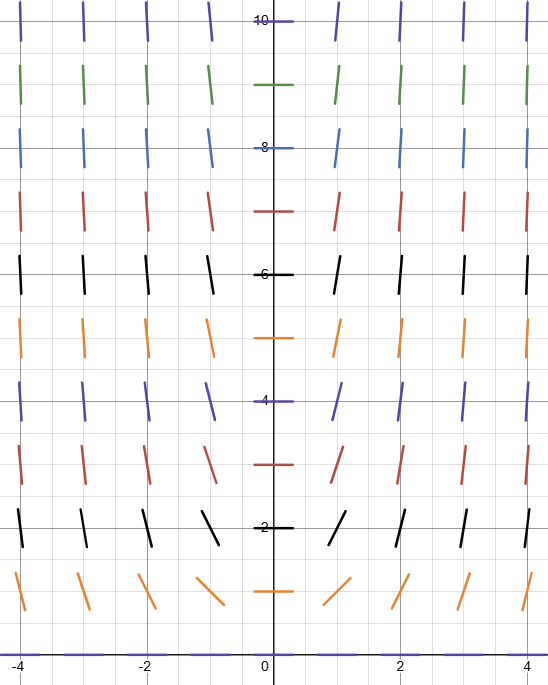
\includegraphics[width=10cm]{F24/Classwork 13/WS y'=xy.png}
        \end{center}

        We still don't have a symbolic expression for $y$ is, but we can use this slope field to estimate evaluations of $y$ at certain points. Use the curve to estimate $y(0)$ and $y(2)$
        \newpage
        \item For the following differential equations, classify them as separable or not. If the equation is separable, separate it.
        \begin{enumerate}
            \item $y'=\dfrac{x}{\sqrt{y}}$\vfill
            \item $y'=\dfrac{\ln(x)+x}{\ln(y)+y}$\vfill
            \item $y'=x+y$\vfill
            \item $y'=ye^{\sin(x)+\cos(y)}$\vfill
            \item $y'=\ln(xy)$\vfill
            \newpage
            \item $y'=\ln(x^{y})$\vfill
            \item $y'=\sin(x^{y})$\vfill
            \item $y'=y\sin(x)+xy$\vfill
            \item $y'=\dfrac{xy+y}{2x-3xy}$\vfill
            \item $y'=xy-2x+y-2$\vfill
        \end{enumerate}
        \newpage
        \item Solve the following separable differential equations
        \begin{enumerate}
            \item $y'=4x^{3}y^{2}$\vfill
            \item $y'=y\cos(x)-x^{3}y$ (assume $y>0$)\vfill
            \item $y'=xy^2-2y^2+x-2$ \vfill
        \end{enumerate}
        
    \end{enumerate}

\end{document}